\skriptsection{Morphological Image Processing (V5, 6, 7)}{627}

  \skriptsubsection{Overview}{662}
  \begin{minipage}{9.5cm}
    Be aware of the $\hat{ }$ which is the reflection!\\
    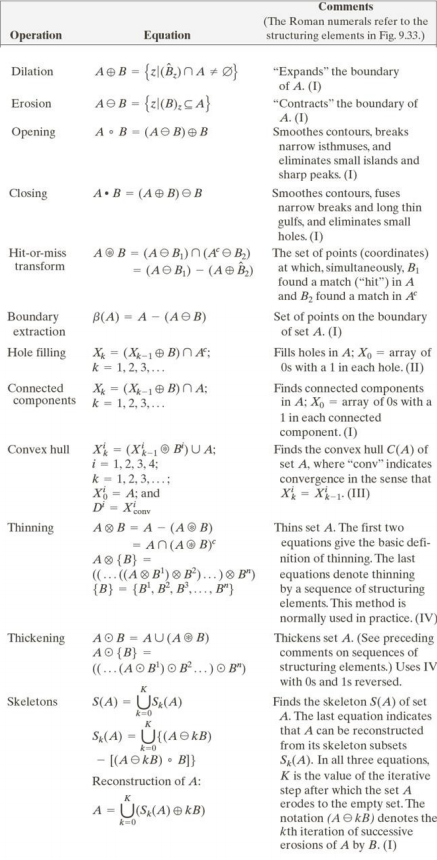
\includegraphics[width=9cm]{./images/morphology_table.png}
  \end{minipage}
  \begin{minipage}{9.5cm}
    Morphological approaches are nonlinear operations on binary or grey images.
    
    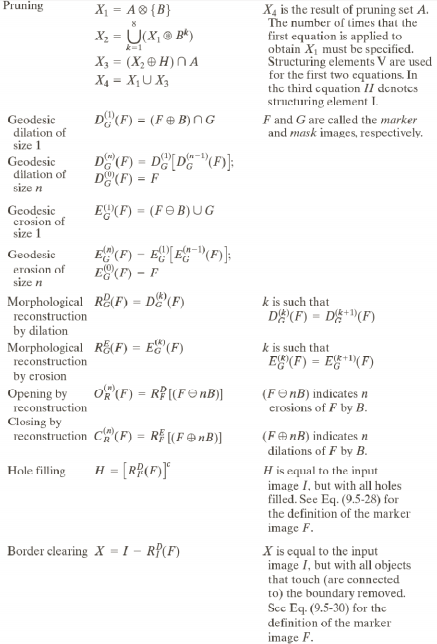
\includegraphics[width=9cm]{./images/morphology_table2.png}   
  \end{minipage}

  \skriptsubsection{Dilation}{633}
  Dilation (dt. wachsen) grows or thickens objects in a binary image. The structure element $H$
  is replicated at every foreground pixel of $I$:\\
  \begin{minipage}{9cm}
    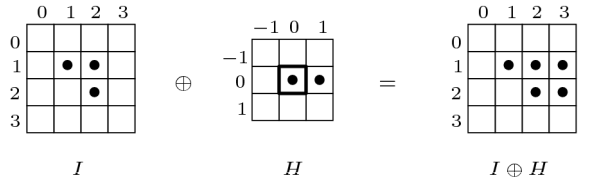
\includegraphics[width=9cm]{./images/dilatation.png}
  \end{minipage}
  \hspace{0.5cm}
  \begin{minipage}{9cm}
    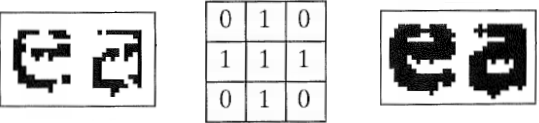
\includegraphics[width=9cm]{./images/dilatation_example.png}
  \end{minipage}
  
  \begin{minipage}{9.5cm}
    \subsubsection{Properties}
    \begin{liste}
      \item $I \oplus H = H \oplus I$
      \item $(I_1 \oplus I_2) \oplus I_3 = I_1 \oplus (I_2 \oplus I_3)$
      \item $I \oplus \delta = \delta \oplus I = I$ ($\delta$ is a neutral object)
    \end{liste}
  \end{minipage}
  \begin{minipage}{9.5cm}
    \subsubsection{Border conditions}
      It is best, to set the pixels at the border with the \textbf{minimum} value of $H$.
  \end{minipage} 

  \skriptsubsection{Erosion}{631}
  Erosion (dt. schrumpfen) shrinks or thins objects in a binary image. Only the pixels of the 
  original image where the structure element is completely encapseled, are in the resulting image.\\
  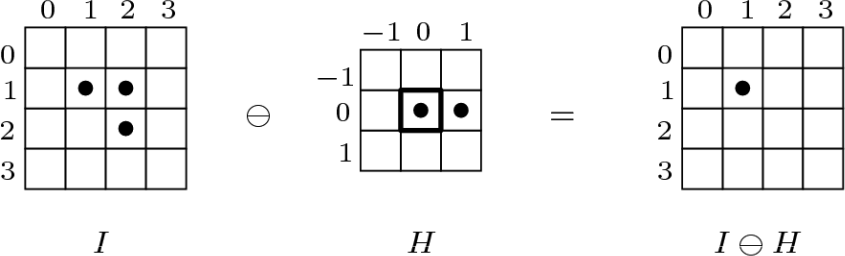
\includegraphics[width=9cm]{./images/erosion.png} 
  \hspace{0.5cm}
  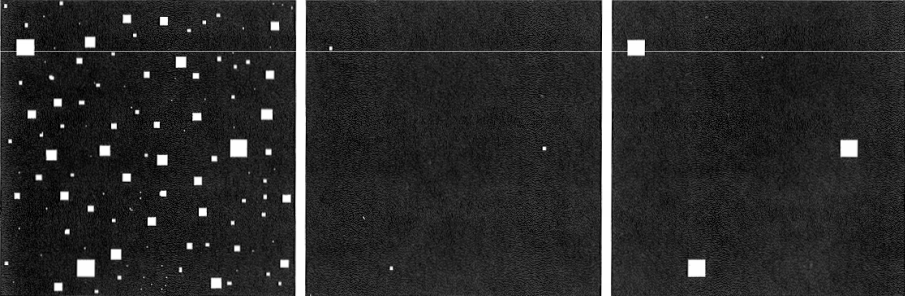
\includegraphics[width=9.5cm]{./images/erosion_example.png}
  \begin{minipage}{9.5cm}
    \subsubsection{Properties}
    \begin{liste}
      \item $I \ominus H \neq H \ominus I$
      \item $(I_1 \ominus I_2) \ominus I_3 \neq I_1 \ominus (I_2 \ominus I_3)$
    \end{liste}
  \end{minipage}
  \begin{minipage}{9.5cm}
    \subsubsection{Border conditions}
      It is best, to set the pixels at the border with the \textbf{maximum} value of $H$.
  \end{minipage}
  
  
  \skriptsubsection{Duality of Erosion and Dilation}{635}
  $(A \ominus B)^c = A^c \oplus \hat{B}$ \qquad
  $(A \oplus B)^c = A^c \ominus \hat{B}$ \qquad with $A^C$ being the complement of $A$ (binary inversion)
  
  
  \begin{minipage}{10cm}
    \skriptsubsection{Opening and Closing}{635}  
      \textbf{Opening}: $A \circ B = (A \ominus B) \oplus B$\\
      Foreground structures which are smaller than $H$ are eliminated by erosion. Dilation lets the
      structures grow back to its original size.  
      
    \textbf{Closing}: $A \bullet B = (A \oplus B) \ominus B$\\
      Holes in the foreground structures are eliminated by dilation. Erosion lets the
      structures shrink back to its original size.
      
    \textbf{Duality}: $(A \bullet B)^c = A^c \circ \hat{B})$, $(A \circ B)^c = A^c \bullet \hat{B})$
    
    \textbf{Properties}:
    \begin{liste}
      \item $A \circ B$, $A \bullet B$ are subsets of $A$
      \item $(A \circ B) \circ B = A \circ B$,  $(A \bullet B) \bullet B = A \bullet B$
    \end{liste}
  \end{minipage}
  \begin{minipage}{9cm}
    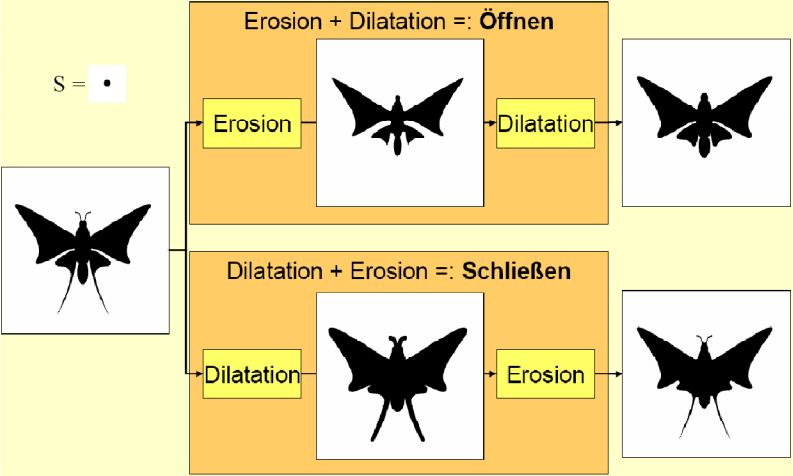
\includegraphics[width=9cm]{./images/morphology_opening_closing.png}
  \end{minipage}
  
  \vspace{1em}
  \begin{minipage}{9.2cm}
    \skriptsubsection{Hit-or-Miss Transform}{640}
      Finds shapes that are bigger than some (small) structure element $D$ and smaller than some 
      (big) second structure element $W$: $A \circledast B = (A \ominus D) \cap (A^c \ominus (W-D))$.
  \end{minipage}
  \hspace{0.6cm}
  \begin{minipage}{9.2cm}
    \skriptsubsection{Boundary Extraction}{642}
      Find difference between original image $A$ and erosion of $A$ with $B$: 
      $\beta(A) = A - (A \ominus B)$.
  \end{minipage}
  
  \vspace{1em}
  \begin{minipage}{9.2cm}
    \skriptsubsection{Hole Filling}{643}
      Fills out any holes (background regions) starting from a starting point: 
      $X_k = (X_{k-1} \oplus B) \cap A^c$ with $X_0$ being an image of same size as $A$ with single 
      pixels as starting point. This is an iterative approach.
      
      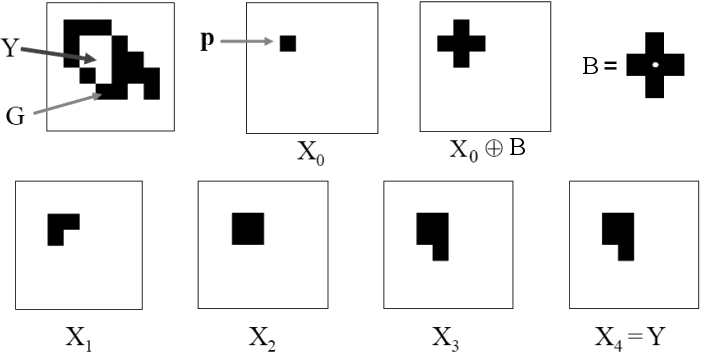
\includegraphics[width=7cm]{./images/morphology_hole_filling.png}
  \end{minipage}
  \hspace{0.6cm}
  \begin{minipage}{9.2cm}
    \skriptsubsection{Connected Components}{645}
      Find objects which are connected: $X_k = (X_{k-1} \oplus B) \cap A$.
      The only difference to hole filling is that here we are looking for foreground pixels instead of
      background pixels.
      \begin{flushright}
        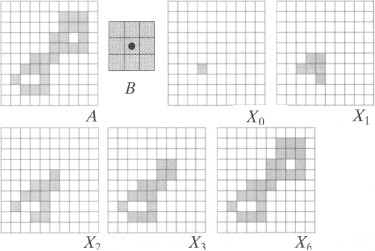
\includegraphics[width=5.5cm]{./images/morphology_connected_components.jpg}
      \end{flushright}
  \end{minipage}
  
  \begin{minipage}{11.5cm}
    \subsection{Other Tools} 
      Convex Hull \formelbuch{647}, Thinning \formelbuch{649}, Thickening \formelbuch{650}, 
      Skeletons \formelbuch{651}, Pruning \formelbuch{654}
      
    \skriptsubsection{Morphological Reconstruction}{656,676}
      Used after opening to grow back pieces of the original image that are connected to the opening.
      
      In addition to the structure element $B$ (block), here a marker image $F$ with starting points and a 
      mask image $G$ are required. $F \subseteq G$. 
  \end{minipage}
  \hspace{0.5cm}
  \begin{minipage}{7cm}
    \begin{flushright}
      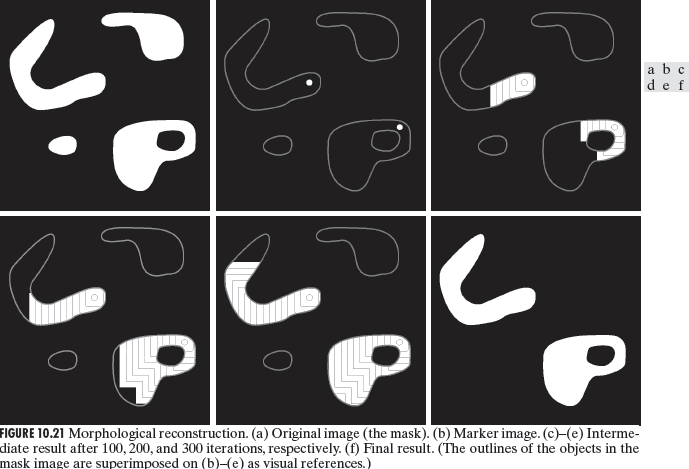
\includegraphics[width=7cm]{./images/morphology_reconstruction.png}
    \end{flushright}
  \end{minipage}
  \vspace{0.5em}
  
  \begin{minipage}{9.2cm}
    \skriptsubsubsection{Geodesic Dilation}{656}
      Init: $D_G^{(n)}(F)=F$ \\
      First it. (size 1): $D_G^{(1)}(F) = (F \oplus B) \cup G$\\
      Recursion (size $n$): $D_G^{(n)}(F) = D_G^{(1)}[D_G^{(n-1)}(F)]$
      
      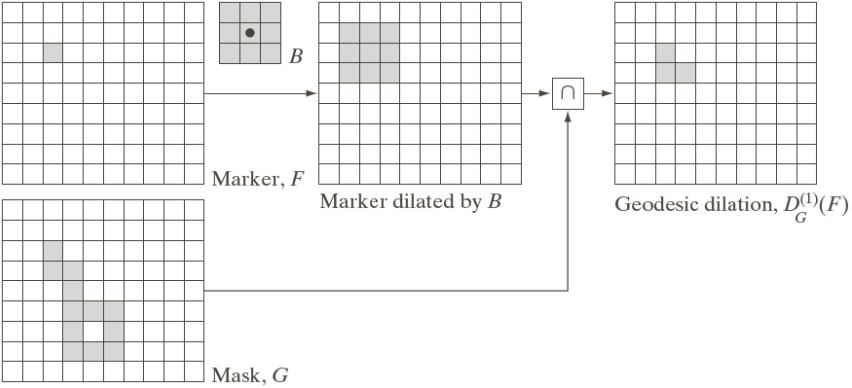
\includegraphics[width=8cm]{./images/morphology_geodesic_dilation.png}
      
    \skriptsubsubsection{Morphological Recon. by Dilation}{658}
      The iterative approach reconstructs the whole object out of a starting point.
      
      $R_G^D(F) = D_G^{(k)}(F)$
      
      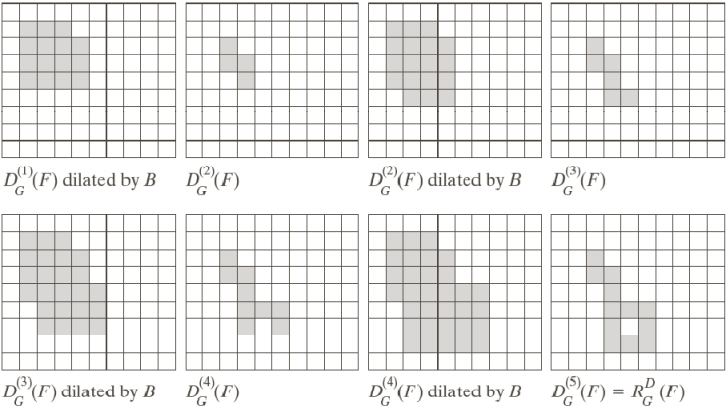
\includegraphics[width=8cm]{./images/morphology_reconstruction_dilation.png}
  \end{minipage}
  \begin{minipage}{9.2cm}
    \skriptsubsubsection{Geodesic Erosion}{657}
      Init: $E_G^{(n)}(F)=F$ \\
      First it. (size 1): $E_G^{(1)}(F) = (F \ominus B) \cap G$\\
      Recursion (size $n$): $E_G^{(n)}(F) = E_G^{(1)}[E_G^{(n-1)}(F)]$
        
      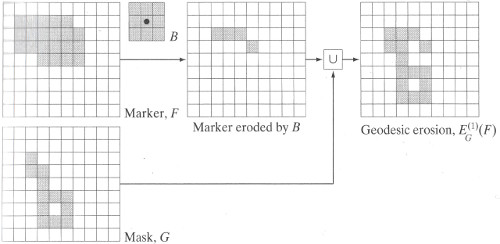
\includegraphics[width=8cm]{./images/morphology_geodesic_erosion.jpg}
      
    \skriptsubsubsection{Morphological Recon. by Erosion}{658}
      Reconstruction by erosion reconstructs holes.
      
      $R_G^E(F) = E_G^{(k)}(F)$
  \end{minipage}
  
  
  \skriptsubsubsection{Sample Applications}{659}
    \subsubsubsection{Opening by Reconstruction}
      Mask $g$ is the input image. The structure element $b$ can be selected to find meaningful starting 
      points (e.g. line with 50 pixels length).
      The marker is then calculated using $f = g \ominus b$.
      Then magic comes into play: The iterative reconstruction uses this equation: $(f \oplus nB) \bigwedge g$
      where $nB$ is the iteration number with 
      $0B = \begin{bmatrix}
      1&1&1\\
      1&1&1\\
      1&1&1\\
      \end{bmatrix}$
      and $\bigwedge$ is the minimum operator.
      This is done until the image is stable (does not change anymore).
      
    \subsubsubsection{Hole Filling} Automatic filling of holes (including starting point seeking)
    
    \subsubsubsection{Border Cleaning} e.g. OCR: All characters which contact the border can be 
    removed
  
  \skriptsubsection{Gray-Scale Morphology}{665}
    Uses function theory instead of set theory (Mengenlehre).
    In particular, the Top-Hat transformation \formelbuch{672} is interesting for shading 
    correction.